% !TeX spellcheck = en_US
\documentclass[11pt]{article}

\usepackage{enumitem}
\usepackage{graphicx}
%opening
\title{Advanced Machine Learning - Assignment 4}
\author{Pranav Kasela \\$846965$}
\date{}

\begin{document}

\maketitle

\section*{Introduction}
The dataset consists of images ($150\times150$) with 6 classes: Forest, Mountains, Buildings, Sea, Glacier and Street (Figure \ref{fig:example}). The data is divided in 14034 training samples and 3000 test samples, the training set is splitted into training and validation (80\%-20\%) during the training to test different hyperparameters.
\begin{figure}[!h]
  \centering
  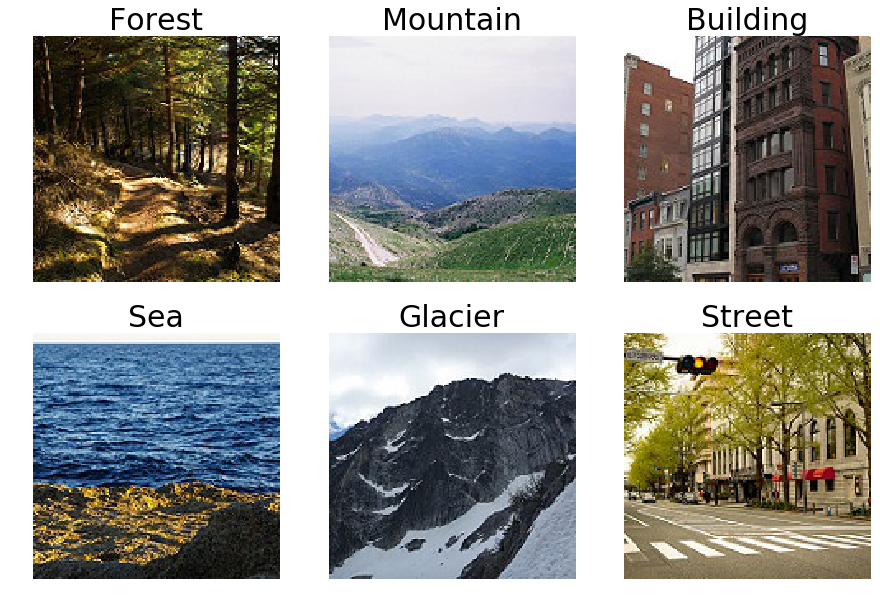
\includegraphics[width=\linewidth, height=6cm]{imgs/samples.png}
  \caption{Example of the 6 classes.}
  \label{fig:example}
\end{figure}

For the assignment the transfer model used is VGG16, the back of the architecture (without the final FC layers) is represented in Figure \ref{fig:VGG16} along with the points where the four cuts are done the features are extracted with a GlobalMaxPooling in all four cuts in order to avoid having a lot of features during the training.
After the feature extraction the machine learning model used is the SVM with linear kernel in all four cases.
\begin{figure}[!h]
  \centering
  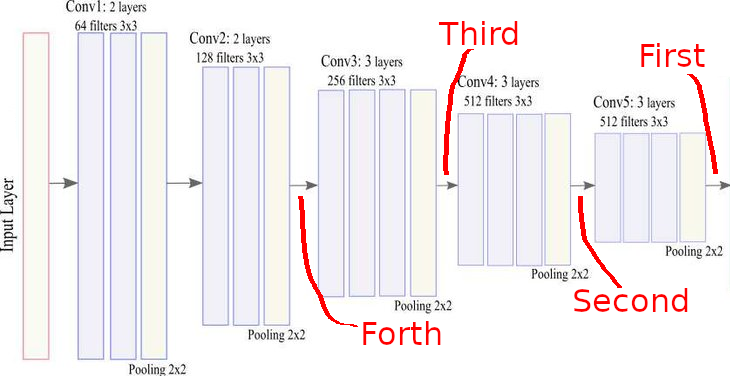
\includegraphics[width=\linewidth, height=5cm]{imgs/VGG16.png}
  \caption{Top of VGG16 Architecture and the cuts for Transfer Learning}
  \label{fig:VGG16}
\end{figure}

\section*{Results}
Both in the First and Second cut the feature extracted are 512, while in the Third and Fourth cut there are 256 and 128 features respectively, these cut are done at each block of the VGG16 (except for  to see how much the classic machine learning classification models are able to distinguish the images based on the the results obtained by VGG16 pretrained on imagenet.\\
Here are the accuracy results using the Support Vector Classifier with linear kernel, the C coefficient is different in all three cases, only the C with the best performance on validation was chosen:
\begin{center}
  \begin{tabular}{|l|c|c|c|}
    \hline
    & Train & Validation & Test\\
    \hline
    First Cut $(C=0.5)$ & 0.949 & 0.899 & 0.894\\
    \hline
    Second Cut $(C=1)$ & 0.958 & 0.908 & 0.903\\
    \hline
    Third Cut $(C=0.5)$ & 0.919 & 0.895 & 0.897\\
    \hline
    Forth Cut $(C=0.1)$ & 0.847 & 0.835 & 0.829\\
    \hline
  \end{tabular}
\end{center}
The best cut seems to be the Second one, since it obtains similar (better) performance when compared to the other cut. In the Forth cut the performance got drastically worse, losing about $11\%$ of accuracy in training and $7\%$ in test and validation compared to the Second Cut.\\
The result could have been expected since there are some classes very similar to the imagenet dataset for example sea-(seashore, coast), street-(street sign), so going deeper in the model will create more interesting features for the classification.


\end{document}
